\chapter{Preliminary Analysis of a Rocket}
The following chapter describes the functionality and structure behind a rocket. The goal is to determine which factors that leads to instability in flight and launch of a rocket. 



The full scale rocket model that will be described consist of,
\begin{itemize}[noitemsep]
\item a payload system.
\item a guidance system.
\item a propulsion system. 
\item a structural system.
\end{itemize}    
The model is seen cf. figure \ref{fig:RocketStructure}.
\begin{figure}[htbp]
	\centering
 	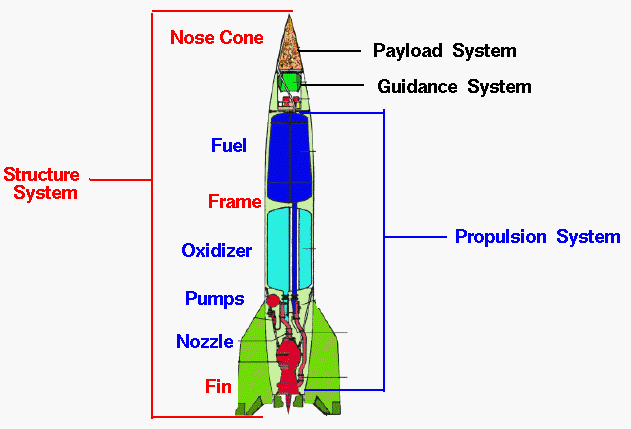
\includegraphics[width=0.65\textwidth]{figures/RocketStructure.png} 
 	\caption{Structure of a full scale rocket.}
 	\label{fig:RocketStructure}
\end{figure}
%https://spaceflightsystems.grc.nasa.gov/education/rocket/rockpart.html

\textbf{Payload System}\\
Most rockets has some form of a payload system. The goal of the payload system is to carry different objects to its wanted destination. The payload can be everything from satellites and astronauts to fireworks depending on the purpose of the rocket. 


\textbf{Guidance System}\\
All rockets that has the goal to be directed or controlled includes a guidance system. The guidance system consist of a processors, sensors, radars, and  a form of wireless communication. Its purpose is to control the stability, direction and rotation of the rocket during launch and in flight. The guidance system is developed based on the understanding of forces acting rocket and its motion. The guidance system in moderne rockets often actuate on the propulsion and nozzle system to correct rotation and direction of the rocket.

\textbf{Propulsion System}\\
The propulsion system of a rocket is the part which thrust the rocket. Thrust is the the main force that makes the rocket launch and fly. All propulsion systems is based on Newton's third law. This means that a propulsion system should be able make a combustion which produces a downwards force high enough to launch the structural system of the rocket. 


\textbf{Structural System}\\
Close to all full scale rockets consist of a structural system. The system consist of the cylindrical body/frame, a nose cone with the payload system and the fins that ensures a stable aerodynamic profile. Though most newer full scales rocket does not rely only on aerodynamics to ensure stability.
\bigbreak   
ss

%All based on https://spaceflightsystems.grc.nasa.gov/education/rocket/rockpart.html


\section{Stability of a Rocket}
Describe why stability is important for a rocket. 
\section{Mechanical System of a Rocket}
Input/output relation of a rocket.
\section{The Inverse Pendulum}
relate the rocket model to a Inverse Pendulum